%------------------------------------------------
\section{MITM \& HTTPS}
%------------------------------------------------

\subsection{MITM}
\begin{frame}
\begin{center}
Le type au millieu.\\

\includegraphics[scale=0.80]{res/mitm}\\
Quelqu'un en position de MITM peut:
\begin{itemize}
    \item Intercepter le traffic
    \item Modifier le traffic
\end{itemize}
\end{center}
\end{frame}



%------------------------------------------------
\subsection{HTTP}
\begin{frame}
\frametitle{HTTP}

\begin{itemize}
    \item HTTP est ni authentifié, ni encrypté.
    \item Certains acteurs peux scrupuleux utilisent ça pour lancer des DDoS massifs
\end{itemize}
\begin{center}
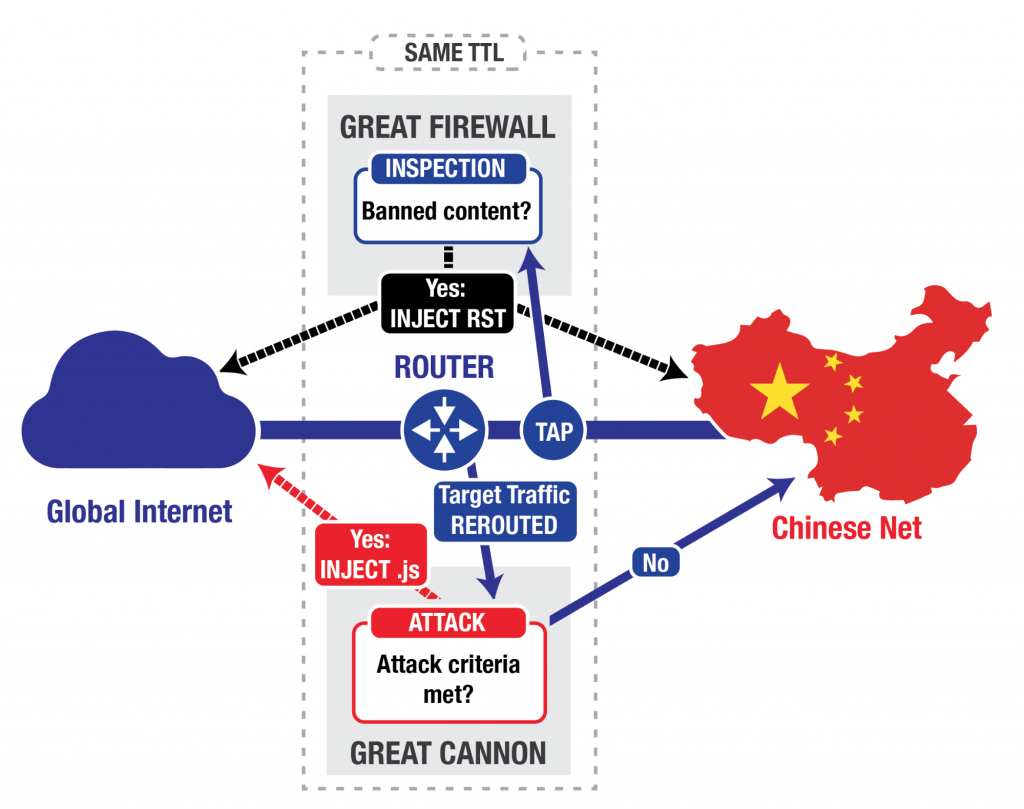
\includegraphics[scale=0.20]{res/great_cannon}
\end{center}
\end{frame}

\note{

    \href{https://arstechnica.com/security/2015/04/meet-great-cannon-the-man-in-the-middle-weapon-china-used-on-github/}{\beamergotobutton{Ars Technica's article on China's "Great Cannon"}}

}


%------------------------------------------------
\subsection{HTTPS}
\begin{frame}
    \frametitle{HTTPS}
    \begin{itemize}
        \item La version "sûre" de HTTP
        \item À la fois encrypté et authentifié
        \item Meilleur système actuel pour protéger le traffic, mais loin d'être idéal 
        \item Depuis l'apparition de "Let's Encrypt", il n'y a plus d'excuse pour ne pas protéger le traffic de son site
    \end{itemize}
\end{frame}

\begin{frame}
    \frametitle{HTTPS: implémentation}
    \begin{itemize}
        \item Crypto Asymétrique pour l'établissement de la connexion
        \item Utilisation de certificats contenant des clefs publiques
        \item Crypto symétrique pour le gros du traffic
    \end{itemize}
\end{frame}

\note{

    \href{http://www.moserware.com/2009/06/first-few-milliseconds-of-https.html}{\beamergotobutton{A nice technical analysis of what happens at the begining of an HTTPS connection}}
    \begin{center}
    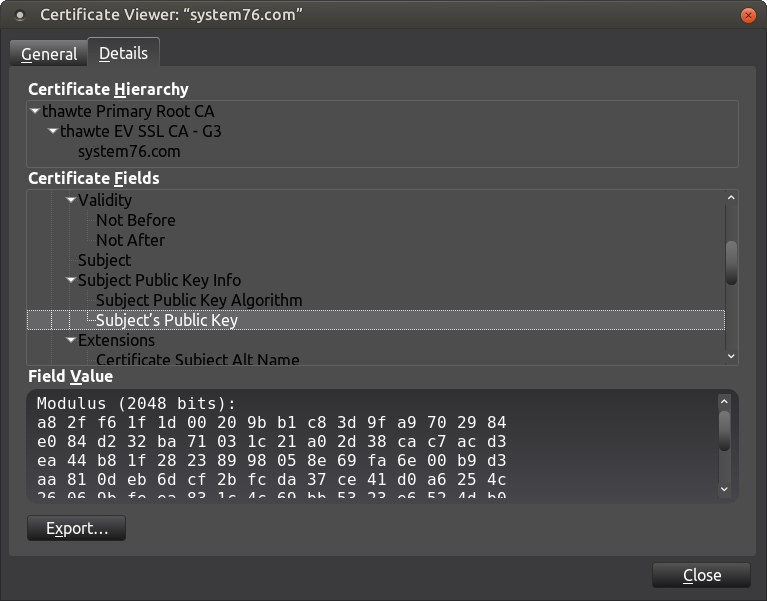
\includegraphics[scale=0.30]{res/https_cert}
    \end{center}
}

\begin{frame}
    \frametitle{HTTPS: Problèmes}
    \begin{itemize}
        \item Basé sur une chaîne de confiance
        \begin{itemize}
            \item Grand nombre de CAs "root"
            \item Contrôle d'un CA 'root' permet de MITM le traffic
            \item Certains CAs ne sont pas dignes de confiance
        \end{itemize}
        \item Approche souvent trop tolérante car
        \begin{itemize}
            \item Les entreprises ont de l'inertie
            \item Sécurité moyenne > Pas de sécurité
        \end{itemize}
    \end{itemize}
\end{frame}












